\chapter{\index{Benutzung}Benutzung}

\section{Einrichtung der Entwicklungsumgebung}
Folgende Schritte sind für die Einrichtung einer Entwicklungsumgebung notwendig

\begin{enumerate}
  \item Installieren der Haskell-Plattform \cite{HasP}
  \vspace*{-0.5em}
  \item Optional \textsf{\$HOME/.cabal/bin} zu der \textsf{Path}-Umgebungsvariablen hinzufügen.
  \vspace*{-0.5em}
  \item Yesod mittels \textsf{cabal install yesod-platform yesod-bin} installieren. Die Installation kann einige Minuten dauern. 
  \vspace*{-0.5em}
  \item Installieren von Git \cite{GitIn}
  \vspace*{-0.5em}
  \item Klonen des Git-Repository mittels \textsf{git clone git@github.com:MaxDaten/ecom.git ecom}. Verzeichnis \textsf{ecom} mit den Quellen wird angelegt.
  \vspace*{-0.5em}
  \item Im \textsf{ecom}-Verzeichnis den Befehl \textsf{cabal install --only-dependencies} ausführen.
  \vspace*{-0.5em}
  \item Mit \textsf{yesod devel} den Entwicklungsserver starten, beenden des Servers mit Enter. 
  \vspace*{-0.5em}
  \item Während der Server läuft, kann der Shop standardmäßig unter der URL \\ \textsf{http://localhost:3000} besucht werden. Das Binding des Servers an einen anderen Port und einen anderen Hostname kann in der Datei \textsf{config/settings.yml} konfiguriert werden.
\end{enumerate}

Die Projektstruktur kann \tblref{tbl:Projektstruktur} entnommen werden.

\begin{table}[h!]
  \centering
  \begin{tabular}{|l|p{12cm}|}
    \hline
    \textsf{src} & Quelldateien der Serverlogik \\
    \hline
    \textsf{static} & Alle Dateien, die nicht vom Server generiert werden (Bilder, css/js Bibliotheken...) \\
    \hline
    \textsf{tools} & Quelldateien für das StateManager Tool (\secpref{sec:StateManager}) \\
    \hline
    \textsf{config} & Definition für Routen und sonstige Konfigurationen \\
    \hline
    \textsf{doc} & Dokumentation \\
    \hline
    \textsf{messages} & Lokalisierungsdateien \\
    \hline
    \textsf{samples} & Produktkatalog und -konfiguration als JSON Dateien für den StateManager \\
    \hline
    \textsf{templates} & html, css, js template-Dateien für die Darstellung der Webseiten \\
    \hline
    \textsf{state} & wird vom Server von acid-sate erstellt. beinhaltet die Persistenz-Dateien. \\
    \hline
  \end{tabular}
  \caption{Projektstruktur}
  \label{tbl:Projektstruktur}
\end{table}

\newpage


\section{Die Navigationsleiste}
Auf jeder Seite ganz oben befindet sich die Navigationsleiste, über die mehrere Funktionen schnell erreicht werden können \figref{fig:Navigationsleiste}. Diese Leiste ist unabhängig von der aktuellen Shopseite immer sichtbar und seine Funktionalitäten stehen damit jederzeit zur Ver\-fü\-gung. Sie beinhaltet von links nach rechts die folgenden Funktionen:
\begin{itemize}
  \item Home (1) \\
        Startseite mit vollständigem Produktkatalog
  \vspace*{-0.5em}
  \item Cat1 bis Cat4 (2) \\
        Anzeige der Produkte einer Kategorie (ohne Funktion in aktueller Version)
  \vspace*{-0.5em}
  \item Suche (3) \\
        Suchen nach spezifischen Produkten (ohne Funktion in aktueller Version)
  \vspace*{-0.5em}
  \item Verwaltung (4) \\
        Verwaltungsmenü (\secpref{sec:Verwaltung})
\end{itemize}
Direkt unterhalb der Navigationsleiste und genau wie diese immer sichtbar, wird angezeigt, ob zurzeit ein Nutzer eingeloggt ist. Ist dies der Fall, so wird zusätzlich sein Name eingeblendet  (siehe lila Kreis). Außerdem  kann er mit der Schaltfläche Abmelden (brauner Kreis) auf der rechten Seite ausgeloggt werden.  Ist kein Nutzer angemeldet, so führt ein Klick auf die Schaltfläche Anmelden zur Nutzerverwaltung (siehe Abschnitt Nutzer). 
Wieder etwas darunter werden Nachrichten zur zuletzt vorgenommenen Aktion angezeigt (rosa Kreis).

\begin{figure}[h!]
  \begin{tikzpicture}
  \pgftext{%
    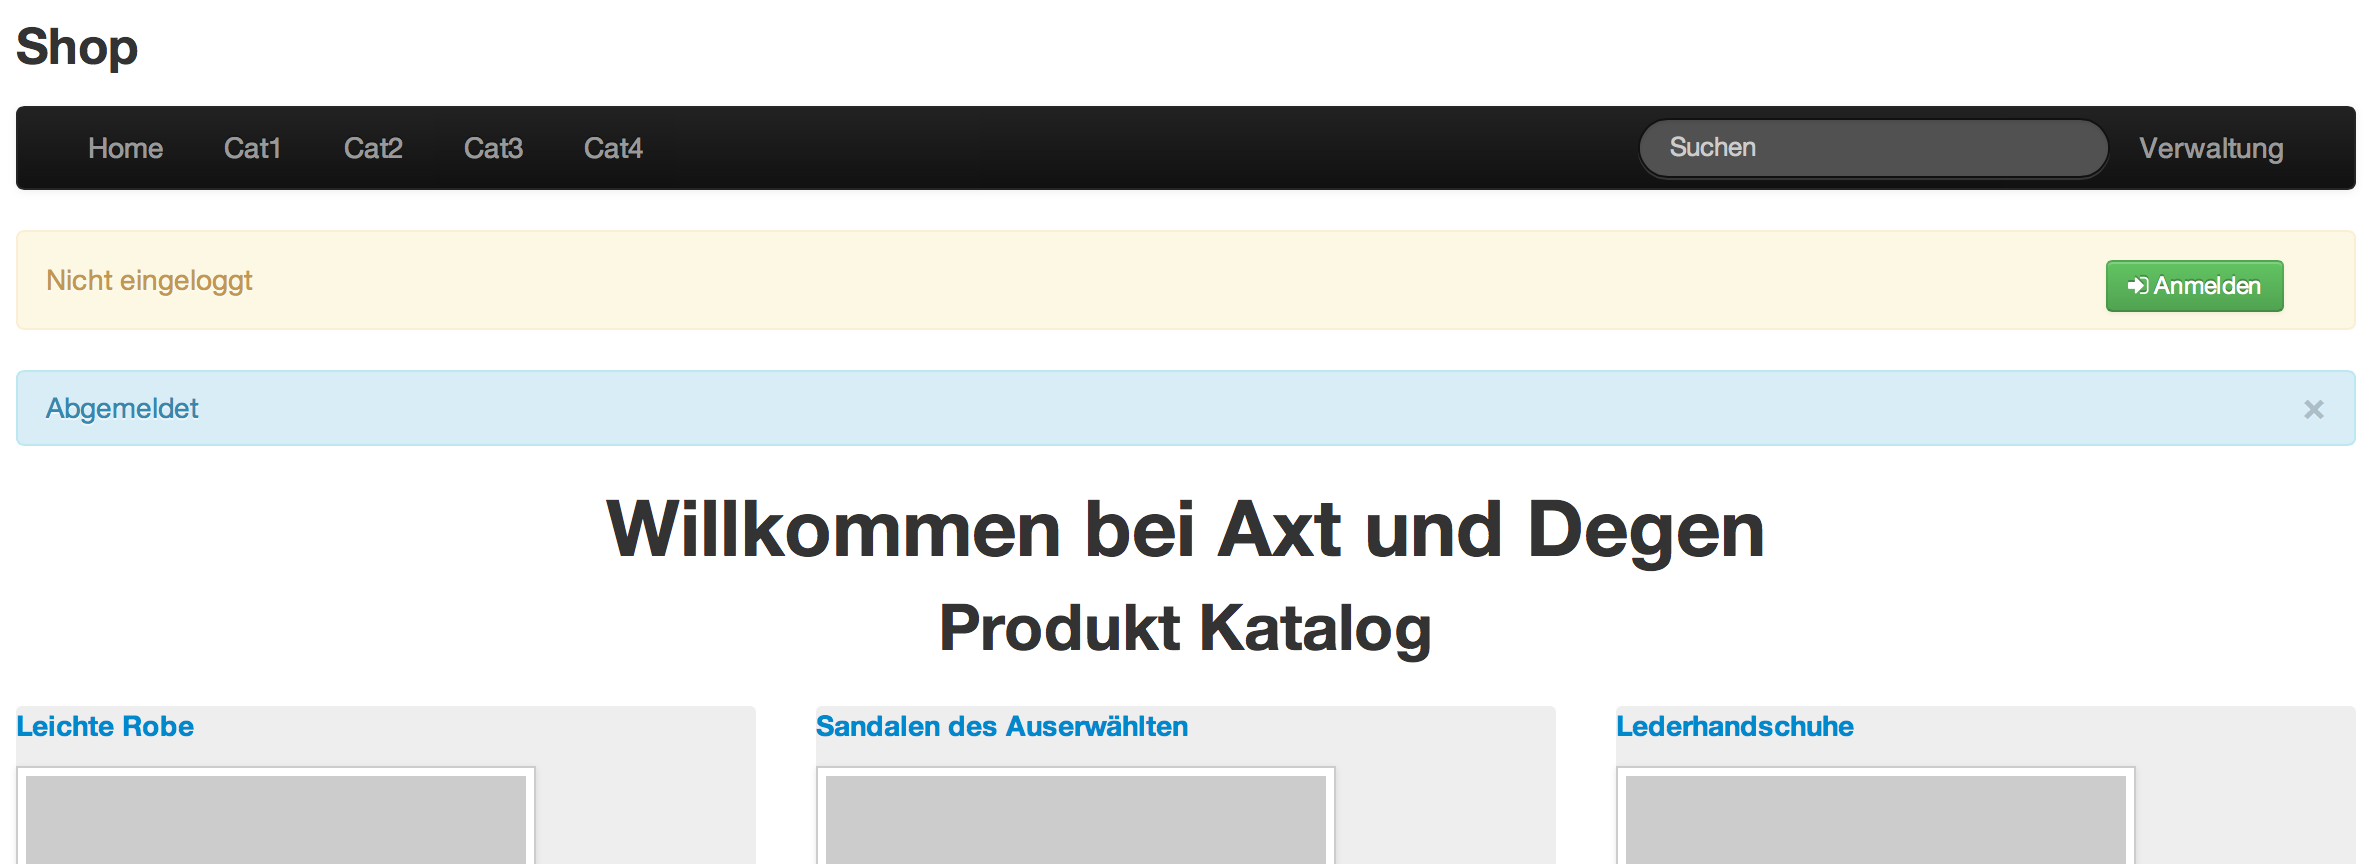
\includegraphics[width=\textwidth]{img/Navi.png}%
  }%
  \node[fill=black, opacity=.5, text opacity=1] at (-7.5,2) [circle] {\bf \tiny \color{white} 1};
  \node[fill=black, opacity=.5, text opacity=1] at (-5,2) [circle] {\bf \tiny \color{white} 2};
  \node[fill=black, opacity=.5, text opacity=1] at (4.5,2) [circle] {\bf \tiny \color{white} 3};
  \node[fill=black, opacity=.5, text opacity=1] at (7.5,2) [circle] {\bf \tiny \color{white} 4};
  % \draw[fill] (0,0) circle [radius=0.1];
  % \draw[help lines] (-8,-4) grid (8,4);
  \end{tikzpicture}
  \centering
  \caption{Navigationsleiste}
  \label{fig:Navigationsleiste}
\end{figure}


\section{Produktkatalog}
Zu Beginn des Shopbesuchs oder durch einen Klick auf eine der Schaltflächen Home in der Navigationsleiste werden alle vorhandenen Produkte des Katalogs angezeigt \figref{fig:Produktkatalog}. Sollte gerade ein Nutzer angemeldet sein, so werden zusätzlich Empfehlungen prä\-sen\-tiert, die auf seinen gemachten Käufen basieren, sofern vorhanden. Über den Schieberegler (1) darüber kann die Reichweite der Empfehlungen erweitert oder eingeschränkt werden. \\
Durch das Anklicken eines Artikels gelangt man auf dessen Produktbeschreibung, siehe auch \chpref{chp:Produktbeschreibung}.

\begin{figure}[h!]
  \begin{tikzpicture}
    \pgftext{%
      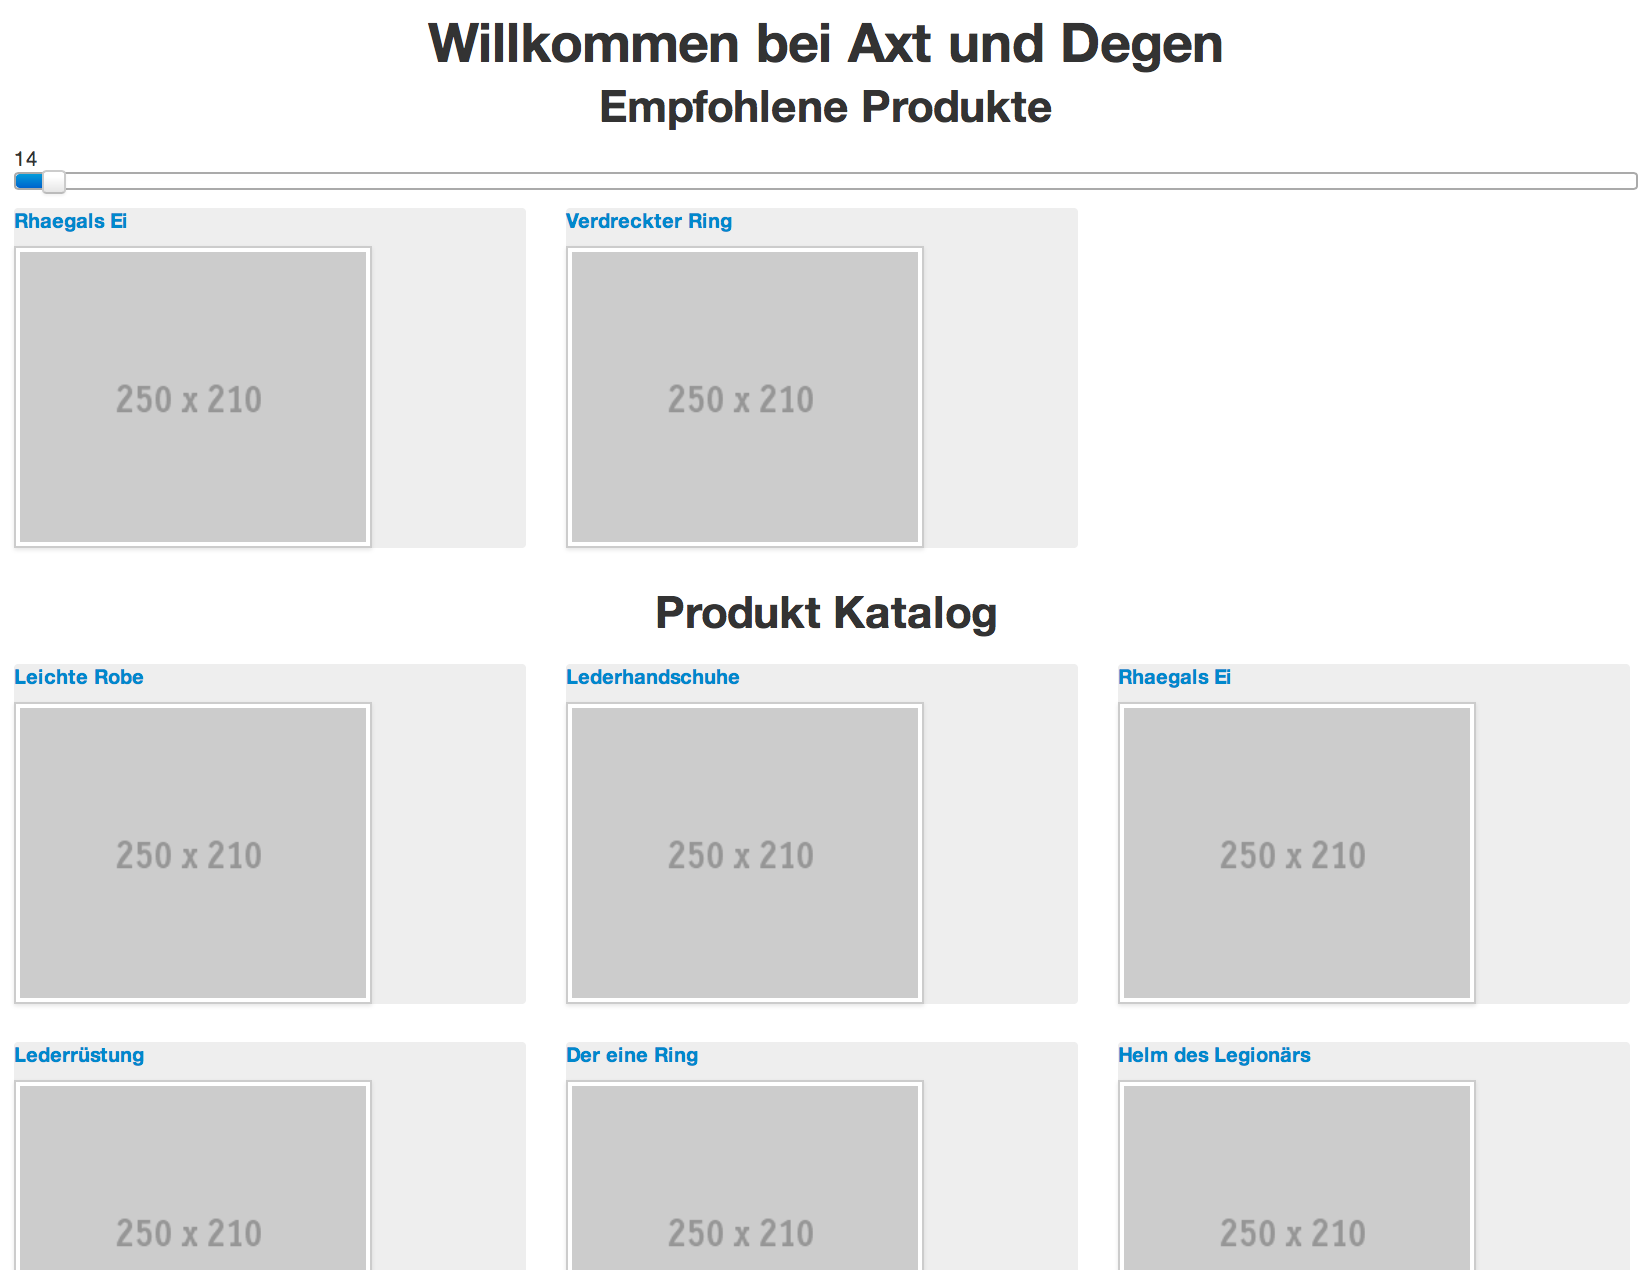
\includegraphics[width=\textwidth]{img/Produktkatalog.png}%
    }%
    \node[fill=black, opacity=.5, text opacity=1] at (0,4.15) [circle] {\bf \tiny \color{white} 1};
    % \draw[fill] (0,0) circle [radius=0.1];
    % \draw[help lines] (-8,-8) grid (8,8);
  \end{tikzpicture}
  \centering
  \caption{Produktkatalog}
  \label{fig:Produktkatalog}
\end{figure}


\section{Verwaltung}
\label{sec:Verwaltung}
Die Administration des Shops kann über das Verwaltungsmenü vorgenommen werden, das über die Navigationsleiste erreichbar ist \figref{fig:Verwaltung}. Es bietet von oben nach unten die folgenden Funktionen:
\begin{itemize}
  \item Produkte verwalten (1) \\
        ruft die Produkteverwaltung auf, siehe \chpref{chp:Produkte}
  \vspace*{-0.5em}
  \item Nutzer verwalten (2) \\
        ruft die Nutzerverwaltung auf, siehe \chpref{chp:Nutzer}
  \item Assoziationen verwalten (3) \\
        ruft die Assoziationsverwaltung auf, siehe \chpref{chp:Assoziationen}
  \vspace*{-0.5em}
\end{itemize}

\begin{figure}[h!]
  \begin{tikzpicture}
    \pgftext{%
      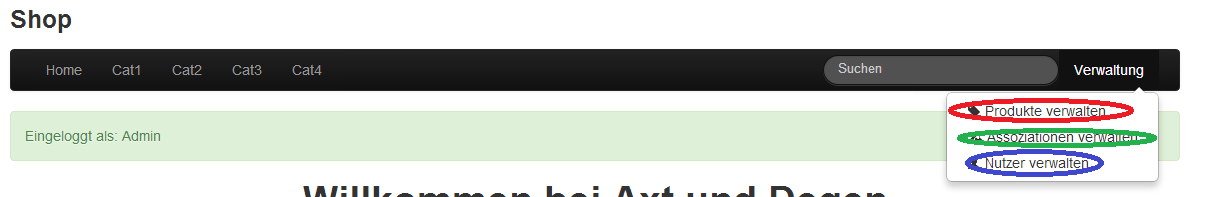
\includegraphics[scale=1]{img/Verwaltung.png}%
    }%
    \node[fill=black, opacity=.5, text opacity=1] at (-0.9,-0.1) [circle] {\bf \tiny \color{white} 1};
    \node[fill=black, opacity=.5, text opacity=1] at (-0.9,-0.8) [circle] {\bf \tiny \color{white} 2};
    \node[fill=black, opacity=.5, text opacity=1] at (-0.9,-1.5) [circle] {\bf \tiny \color{white} 3};
    % \draw[fill] (0,0) circle [radius=0.1];
    % \draw[help lines] (-6,-6) grid (6,6);
  \end{tikzpicture}
  \centering
  \caption{Verwaltung}
  \label{fig:Verwaltung}
\end{figure}


\section{Produkte}
\label{chp:Produkte}
Die Verwaltung der zum Verkauf stehenden Produkte erfolgt über die Produkteverwaltung, die über das Verwaltungsmenü erreichbar ist. Eine Tabelle zeigt alle vorhandenen Produkte auf \figref{fig:Produktverwaltung}. Jede Tabellenzeile ist anklickbar, um direkt zur entsprechenden Produktbeschreibung zu gelangen, siehe dazu auch \chpref{chp:Produktbeschreibung}. Produkte können bearbeitet (2) oder gelöscht werden (3).

\begin{figure}[h!]
  \begin{tikzpicture}
    \pgftext{%
      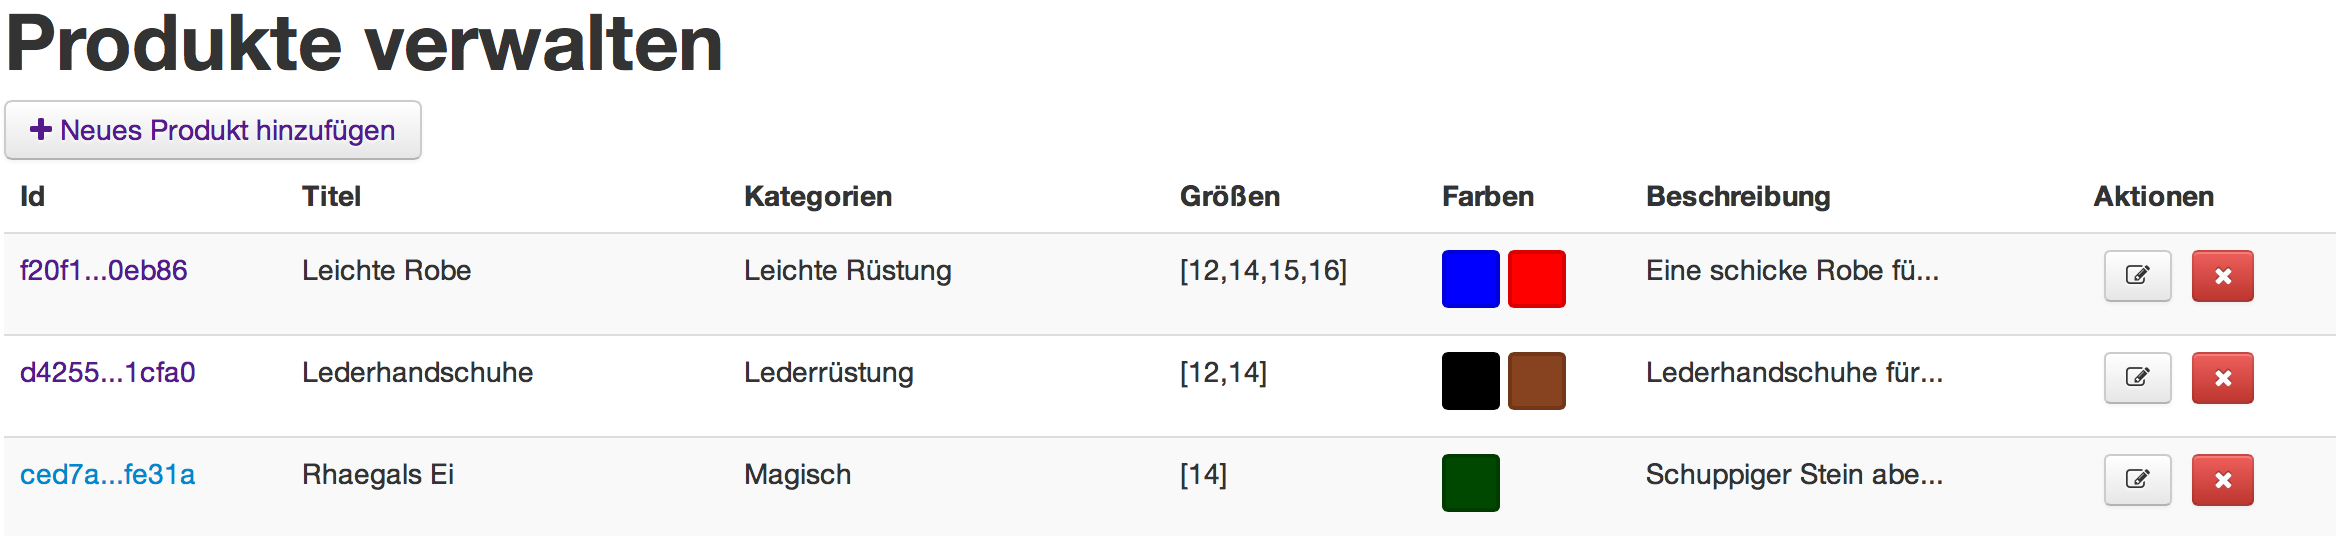
\includegraphics[width=\textwidth]{img/Produkte.png}
    }
    \node[fill=black, opacity=.5, text opacity=1] at (-4.7,0.9) [circle] {\bf \tiny \color{white} 1};
    \node[fill=black, opacity=.5, text opacity=1] at (5.75,-0.05) [circle] {\bf \tiny \color{white} 2};
    \node[fill=black, opacity=.5, text opacity=1] at (7.4,-0.05) [circle] {\bf \tiny \color{white} 3};
    % \draw[fill] (0,0) circle [radius=0.1];
    % \draw[help lines] (-6,-6) grid (6,6);
  \end{tikzpicture}
  \centering
  \caption{Produktverwaltung}
  \label{fig:Produktverwaltung}
\end{figure}
\text{}\vspace*{-1em}\\
Über die Schaltfläche \textit{Neues Produkt hinzufügen} (1) gelangt man zur Produkteeingabemaske, über die neue Produkte in den Shop eingebracht werden können. Dafür müssen alle Felder entsprechend der gewünschten Produktspezifikationen ausgefüllt werden. Kategorien, Größen und Farben müssen in einer kommaseparierten Liste (CSV\nomenclature{CSV}{Comma-Separated Values}) eingegeben werden, Farben werden nur als Hex-Werte mit führendem Hash akzeptiert (\figref{fig:Produktformular})

\begin{figure}[h!]
  \centering
  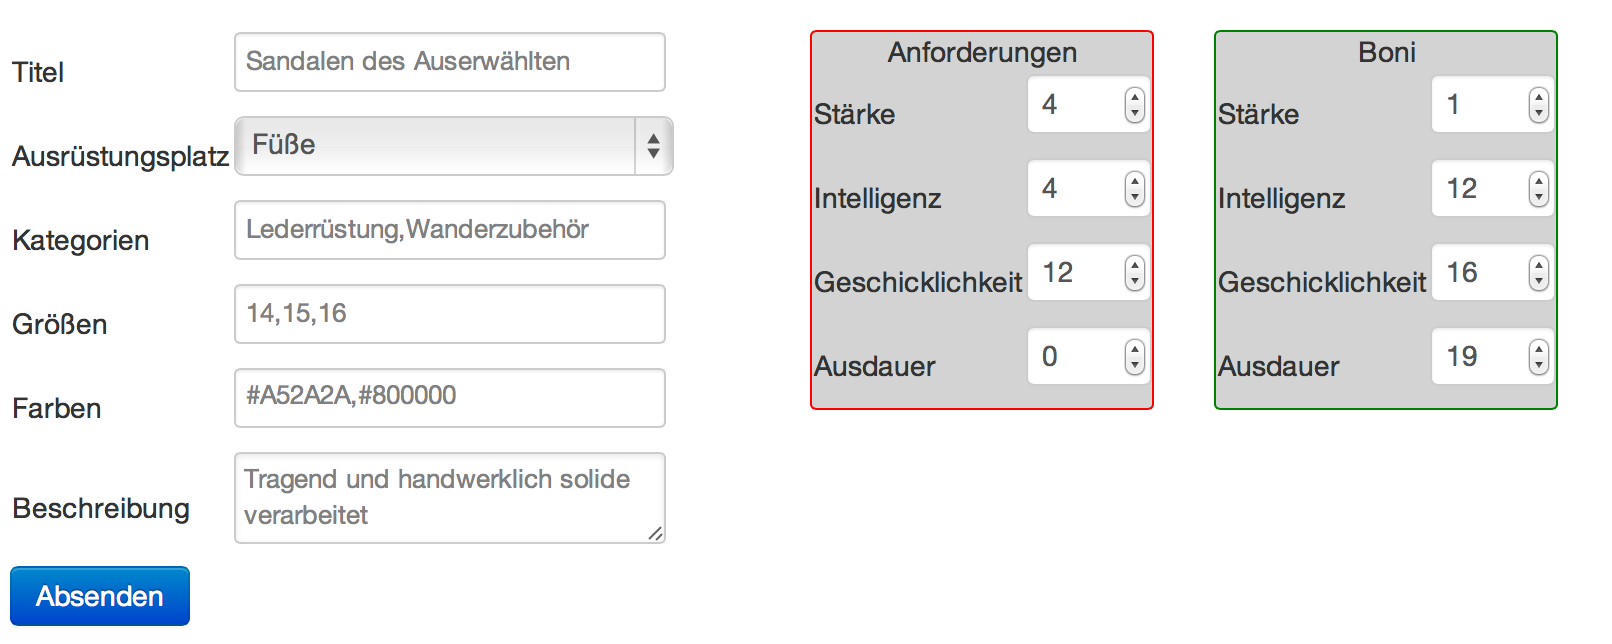
\includegraphics[width=\textwidth]{img/Produktformular.png}
  \caption{Produktformular}
  \label{fig:Produktformular}
\end{figure}

\section{Assoziationen}
\label{chp:Assoziationen}
Die Kategorien, denen Produkte angehören können, lassen sich mit der Hilfe von Assoziationen koppeln. Dadurch werden Artikel dieser Kategorien als zueinander zu\-ge\-hö\-rig definiert und so in der Produktbeschreibung \chpref{chp:Produktbeschreibung} dargestellt. Dies erleichtert es, zusammengehörige Produkte zu erkennen und zu kaufen. Diese Kategorieassoziationen lassen sich in der Assosiationsverwaltung definieren, die über das Verwaltungsmenü erreichbar ist. In dieser werden die vorhandenen Kopplungen in einer Tabelle dargestellt \figref{fig:Assoziationen}. Assoziationen lassen sich bearbeiten (\ref{fig:Assoziationen}.2) oder löschen (\ref{fig:Assoziationen}.3). \\

\begin{figure}[h!]
  \begin{tikzpicture}
    \pgftext{%
      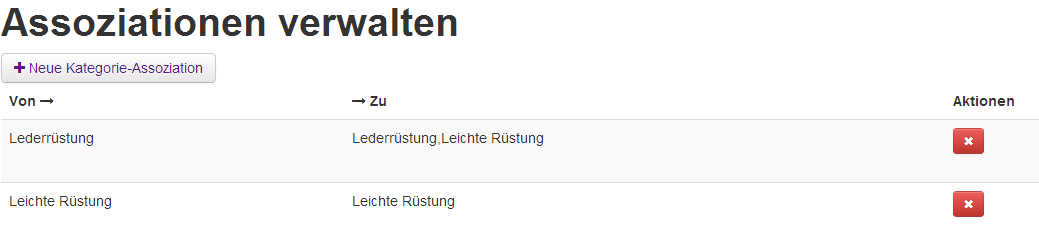
\includegraphics[width=\textwidth]{img/Assoziationen.png}
    }
    \node[fill=black, opacity=.5, text opacity=1] at (-4.3,1.4) [circle] {\bf \tiny \color{white} 1};
    \node[fill=black, opacity=.5, text opacity=1] at (5.2,0.4) [circle] {\bf \tiny \color{white} 2};
    \node[fill=black, opacity=.5, text opacity=1] at (6.9,0.4) [circle] {\bf \tiny \color{white} 3};
    % \draw[fill] (0,0) circle [radius=0.1];
    % \draw[help lines] (-6,-6) grid (6,6);
  \end{tikzpicture}
  \centering
  \caption{Assoziationen}
  \label{fig:Assoziationen}
\end{figure}
\text{}\vspace*{-1em}\\
Über die Schaltfläche \textit{Neue Kategorie-Assoziation}(\ref{fig:Assoziationen}.1) gelangt man zur Asso\-zia\-tionen\-ein\-ga\-be\-mas\-ke. Um darüber neue Assoziationen anzulegen, müssen die beiden Felder \textit{Von} und \textit{Zu} ausgefüllt werden. Im ersten Feld wird eine Kategorie eingetragen und im zweiten eine kommaseparierte Liste (CSV) aus beliebig vielen Kategorien, zu denen eine Kopplung von der Kategorie im ersten Feld aufgebaut werden soll. Kategorien sind nicht automatisch selbstreferenzierend. Soll eine Kategorie sich in einer Assoziation selbst referenzieren, so muss diese ebenfalls im zweiten Feld stehen.


\section{Nutzer}
\label{chp:Nutzer}
Die Administration der im Shopsystem registrierten Nutzer erfolgt über die Nutzerverwaltung, die über das Verwaltungsmenü erreichbar ist. Eine Tabelle listet alle im System vorhandenen Nutzer auf \figref{fig:Nutzer}.

Folgende Aktionen sind möglich:
\begin{itemize}
  \item Nutzerdetails aufrufen (\ref{fig:Nutzer}.2) \figref{fig:Nutzerdetails}
  \vspace*{-0.5em}
  \item als entsprechender Nutzer einloggen (\ref{fig:Nutzer}.3)
  \vspace*{-0.5em}
  \item vollständigen Kauf-Verlauf des Nutzers löschen (\ref{fig:Nutzer}.4)
  \vspace*{-0.5em}
  \item Nutzer löschen (\ref{fig:Nutzer}.5)
\end{itemize}

\begin{figure}[h!]
  \begin{tikzpicture}
    \pgftext{%
      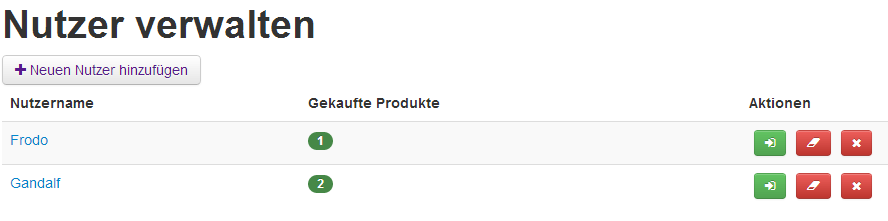
\includegraphics[width=\textwidth]{img/Nutzer.png}
    }
    \node[fill=black, opacity=.5, text opacity=1] at (-4.3,1.4) [circle] {\bf \tiny \color{white} 1};
    \node[fill=black, opacity=.5, text opacity=1] at (-5.3,0.35) [circle] {\bf \tiny \color{white} 2};
    \node[fill=black, opacity=.5, text opacity=1] at (4.2,0.55) [circle] {\bf \tiny \color{white} 3};
    \node[fill=black, opacity=.5, text opacity=1] at (5.05,0.55) [circle] {\bf \tiny \color{white} 4};
    \node[fill=black, opacity=.5, text opacity=1] at (5.9,0.55) [circle] {\bf \tiny \color{white} 5};
    % \draw[fill] (0,0) circle [radius=0.1];
    % \draw[help lines] (-6,-6) grid (6,6);
  \end{tikzpicture}
  \centering
  \caption{Nutzer}
  \label{fig:Nutzer}
\end{figure}
\text{}\vspace*{-1em}\\
Die Nutzerdetails \figref{fig:Nutzerdetails} zeigen die Attribute des Nutzers und seine Kaufhistorie an. Über die Schaltfläche oberhalb der Attributwerte (1) können diese ge\-än\-dert werden. Die Bedeutungen der Spalten der Tabelle der gekauften Produkte entsprechen den gleichnamigen Spalten der Tabelle aus der Produkteverwaltung, siehe auch \chpref{chp:Produkte}. Durch einen Klick auf die \textit{Löschen}-Schaltfläche (2) in der Spalte \textit{Aktionen} wird das dazugehörige Produkt gelöscht. Die Produkttitel sind anklickbar und führen direkt zur dazugehörigen Produktbeschreibung, siehe \chpref{chp:Produktbeschreibung}.

Über die Schaltfläche \textit{Neuen Nutzer}(1) hinzufügen gelangt man zur Nutzereingabemaske, über die neue Nutzer im System registriert werden können. Dafür müssen alle Felder ausgefüllt werden \figref{fig:Nutzerformular}.
\begin{figure}[h!]
  \begin{tikzpicture}
    \pgftext{%
      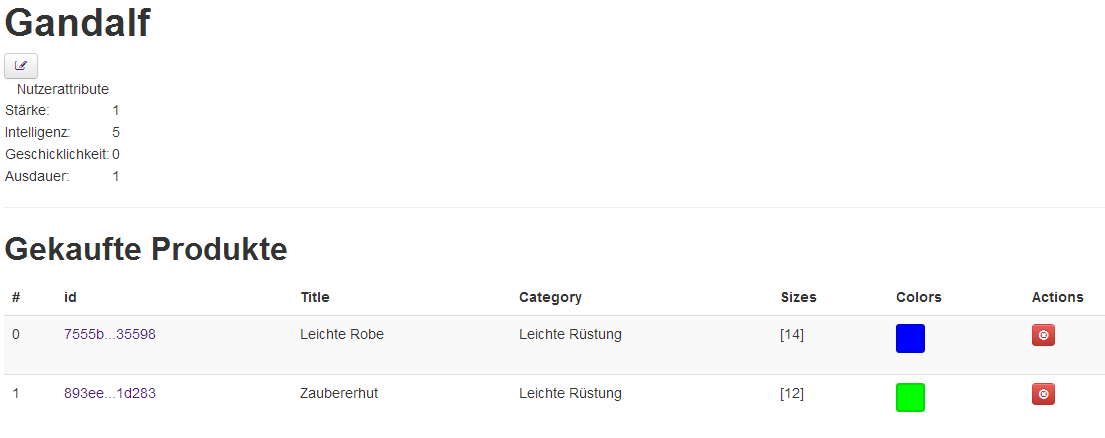
\includegraphics[width=\textwidth]{img/Nutzerdetails.png}
    }
    \node[fill=black, opacity=.5, text opacity=1] at (-6.8,1.7) [circle] {\bf \tiny \color{white} 1};
    \node[fill=black, opacity=.5, text opacity=1] at (5.7,-2) [circle] {\bf \tiny \color{white} 2};
    % \draw[fill] (0,0) circle [radius=0.1];
    % \draw[help lines] (-6,-6) grid (6,6);
  \end{tikzpicture}
  \centering
  \caption{Nutzerdetails}
  \label{fig:Nutzerdetails}
\end{figure}

\begin{figure}[h!]
  \centering
  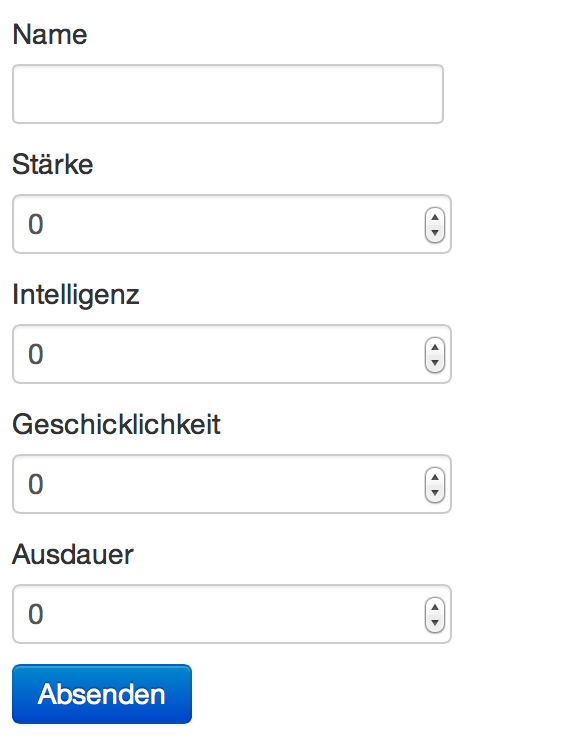
\includegraphics[scale=0.5]{img/Nutzerformular.png}
  \caption{Nutzerformular}
  \label{fig:Nutzerformular}
\end{figure}

\newpage

\section{Produktbeschreibung}
\label{chp:Produktbeschreibung}
Jedes Produkt besitzt eine eigene Seite \figref{fig:Produktbeschreibung}, durch die es präsentiert wird. Außerdem kann es über diese gekauft werden. Jede Produktbeschreibung besteht aus den folgenden Bestandteilen:
\begin{itemize}
  \item Titel (1)
  \vspace*{-0.5em}
  \item Bild des Produktes (2)
  \vspace*{-0.5em}
  \item Beschreibung des Produktes (3)
  \vspace*{-0.5em}
  \item durch das Tragen des Produktes gewährte Attributsboni  (4)
  \vspace*{-0.5em}
  \item Attributswerte, die ein Nutzer besitzen muss, um das Produkt tragen zu können (5)
  \vspace*{-0.5em}
  \item Ausrüstungsplatz, an dem das Produkt getragen wird (6)
  \vspace*{-0.5em}
  \item Drop-Down-Menü, um die gewünschte Größe auszuwählen (7)
  \vspace*{-0.5em}
  \item Radioboxen, um die gewünschte Farbe auszuwählen (8)
  \vspace*{-0.5em}
  \item Schaltfläche zum Kaufen des Produktes (9)
  \vspace*{-0.5em}
  \item mit dem aktuellen Produkt in Verbindung stehende andere Artikel (10)
\end{itemize}
Um ein Produkt zu erwerben, müssen erst Größe und Farbe ausgewählt werden, bevor die Kaufen-Schaltfläche bestätigt wird. Ansonsten erscheint eine Fehlermeldung. Durch Klicken auf die zugehörigen Produkte wird zu deren jeweiliger Produktbeschreibung gewechselt.

\begin{figure}[h!]
  \begin{tikzpicture}
    \pgftext{%
      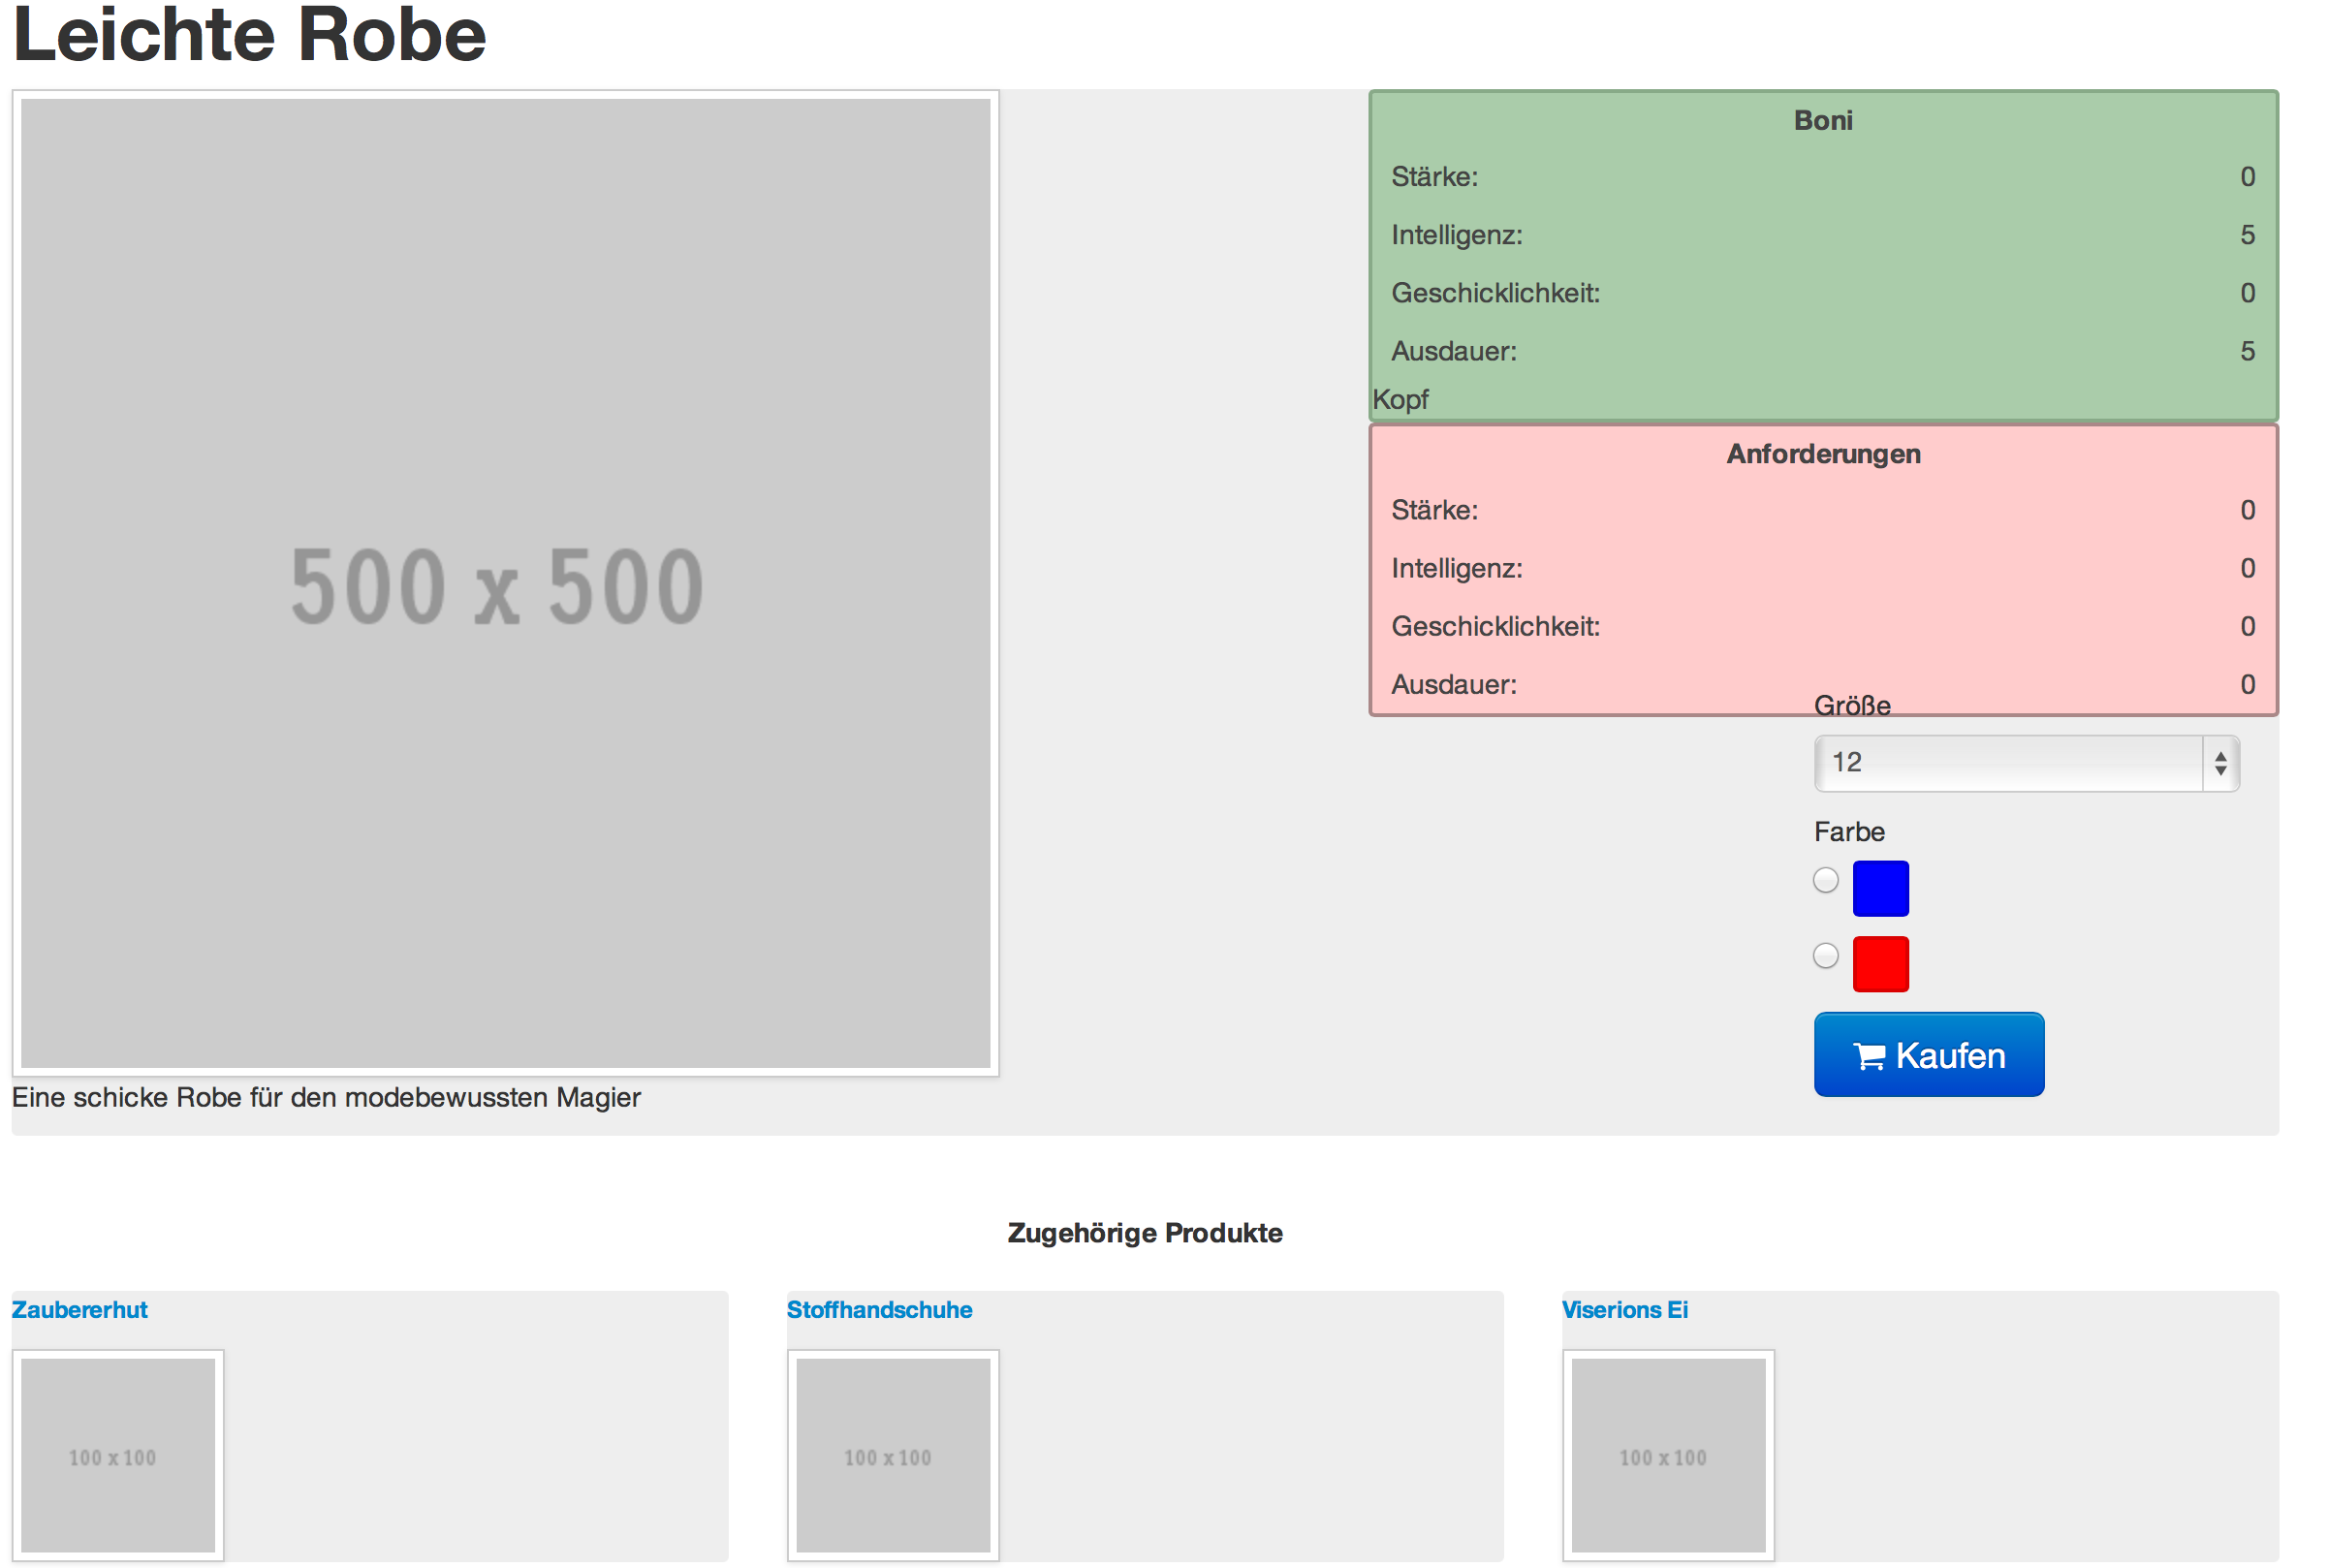
\includegraphics[width=\textwidth]{img/Produktbeschreibung.png}
    }
    \node[fill=black, opacity=.5, text opacity=1] at (-4,5) [circle] {\bf \tiny \color{white} 1};
    \node[fill=black, opacity=.5, text opacity=1] at (-4.5,1.25) [circle] {\bf \tiny \color{white} 2};
    \node[fill=black, opacity=.5, text opacity=1] at (-3,-2) [circle] {\bf \tiny \color{white} 3};
    \node[fill=black, opacity=.5, text opacity=1] at (4,3.5) [circle] {\bf \tiny \color{white} 4};
    \node[fill=black, opacity=.5, text opacity=1] at (4,1.5) [circle] {\bf \tiny \color{white} 5};
    \node[fill=black, opacity=.5, text opacity=1] at (1,2.5) [circle] {\bf \tiny \color{white} 6};
    \node[fill=black, opacity=.5, text opacity=1] at (4,0.2) [circle] {\bf \tiny \color{white} 7};
    \node[fill=black, opacity=.5, text opacity=1] at (4,-0.8) [circle] {\bf \tiny \color{white} 8};
    \node[fill=black, opacity=.5, text opacity=1] at (4,-1.8) [circle] {\bf \tiny \color{white} 9};
    \node[fill=black, opacity=.5, text opacity=1] at (0,-4) [circle] {\bf \tiny \color{white} 10};
    % \draw[fill] (0,0) circle [radius=0.1];
    % \draw[help lines] (-6,-6) grid (6,6);
  \end{tikzpicture}
  \centering
  \caption{Produktbeschreibung}
  \label{fig:Produktbeschreibung}
\end{figure}


\section{StateManager}
\label{sec:StateManager}
Zusammen mit der Shopsoftware wird das Programm StateMananger ausgeliefert. Mit seiner Hilfe können die Produkte und Assoziationen in der Shopdatenbank auch bei nicht laufendem Server selektiv betrachtet, als JSON importiert oder exportiert werden. Die exportierten Dateien finden sich im Ordner \textsf{exports} im \textsf{ecom}-Verzeichnis. \\
Der StateManager lässt sich über die Kommandozeile aus dem ecom-Verzeichnis heraus bedienen. Der Befehl \textsf{runhaskell -isrc tools/StateManger.hs --help} liefert weitere Informationen zu seiner Benutzung. 